\chapter{PaperMVVB additions}

%COFI -- chapter outline and flow integration\\


\section{Literature}
Schwenn1983 intro -> sw-averaging comment (beer and wine)\\
see Hellinger2013 p.1353\\
see astro70/CGAUSS/dropbox\_presis/... (presi 1.07 Inside Helios-Origins and Evolution-Salem.ppt -> Helios reloaded; radial functions for all parameters)\\
see Balogh1999 from p. 162 (Helios CIR results)\\
see Marsch1999... (model constraints)\\
model boundary condition: continuity of mass flux\\
On solar wind acceleration and SPP proposition: McComas2007\\

Motivational question: What is the evolution of the solar wind parameters/structures before arriving at Earth?\\
what is meant by the term evolution?\\


\section{Seasonal solar wind variations}
seasonal variation by month\\
quantify variation amplitudes\\

see \autoref{fig:OMNI_monthly_freq_V_gps}
\begin{figure}[htb]
	\centering
	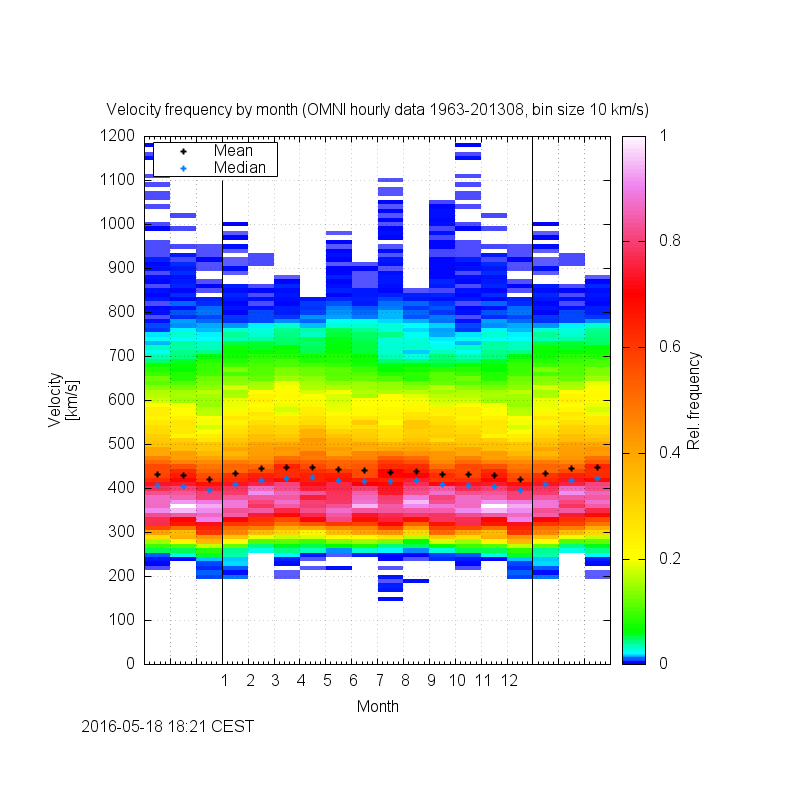
\includegraphics[width=0.3\textwidth]{images/gnuplots/OMNI_monthly_freq_V_gps.png}
	\caption{Diagram of the velocity frequency by month for the period 1963/01--2013/08. Mean and median values are shown as well.}
	\label{fig:OMNI_monthly_freq_V_gps}
\end{figure}

see \autoref{fig:OMNI_monthly_freq_B_a_gps}
\begin{figure}[htb]
	\centering
	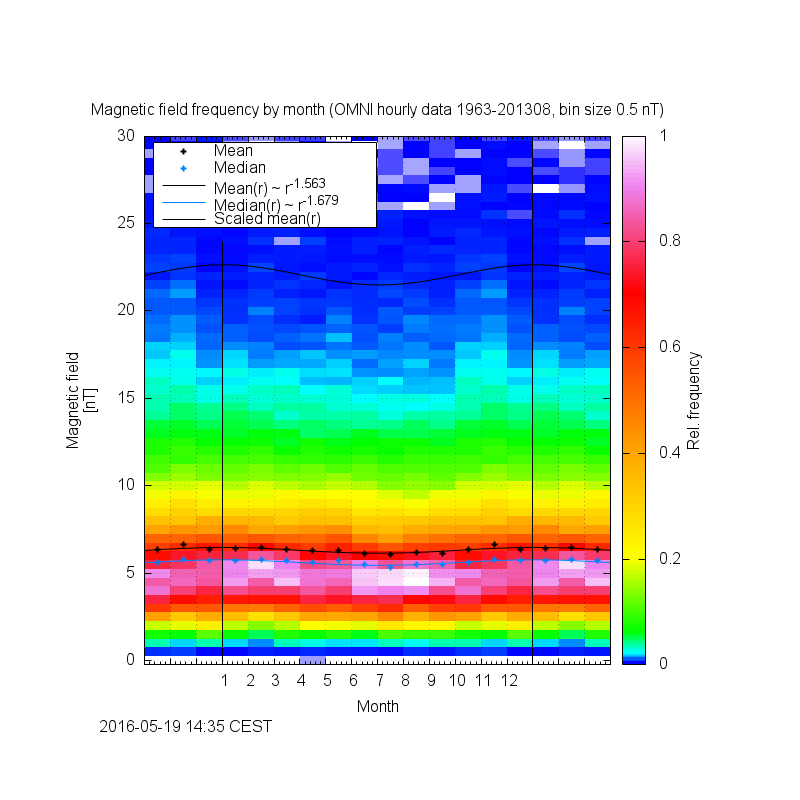
\includegraphics[width=0.3\textwidth]{images/gnuplots/OMNI_monthly_freq_B_a_gps.png}
	\caption{Diagram of magnetic field frequency by month for the period 1963/01--2013/08. Mean and median values are shown as well as the expected course from the solar distance variation (obtained from Helios data).}
	\label{fig:OMNI_monthly_freq_B_a_gps}
\end{figure}

derived exponent values from simple trigonometric fit on monthly values:\\
$c_N = -2.234$\\
maybe figure?\\

expected influence from Earth's perihelion/aphelion (see Appendix...) distance vs observations\\
we expect for the proton density (scaling law $N(r) = 7.6~\text{cm}^{-3} \cdot r^{-2}$):\\
N(0.983~au) = 7.9~cm$^{-3}$\\
N(1~au) = 7.6~cm$^{-3}$\\
N(1.017~au) = 7.3~cm$^{-3}$\\
we expect for the magnetic field strength (scaling law $\propto r^{-1.6}$):\\
B(0.983~au) = 6.3~nT\\
B(1~au) = 6.1~nT\\
B(1.017~au) = 5.9~nT\\


\section{Latitude dependency}
refer to Ulysses figure...\\
Ulysses swoops polar plots...\\
see Schwenn1990's~Fig.~3.14\\
see also \citet{Schwenn1990} p.~127\\
see also \citet{Richardson1995}\\

latitude; see \autoref{fig:latitude_frequency_4_thesis_plot}
\begin{figure}[htb]
	\centering
	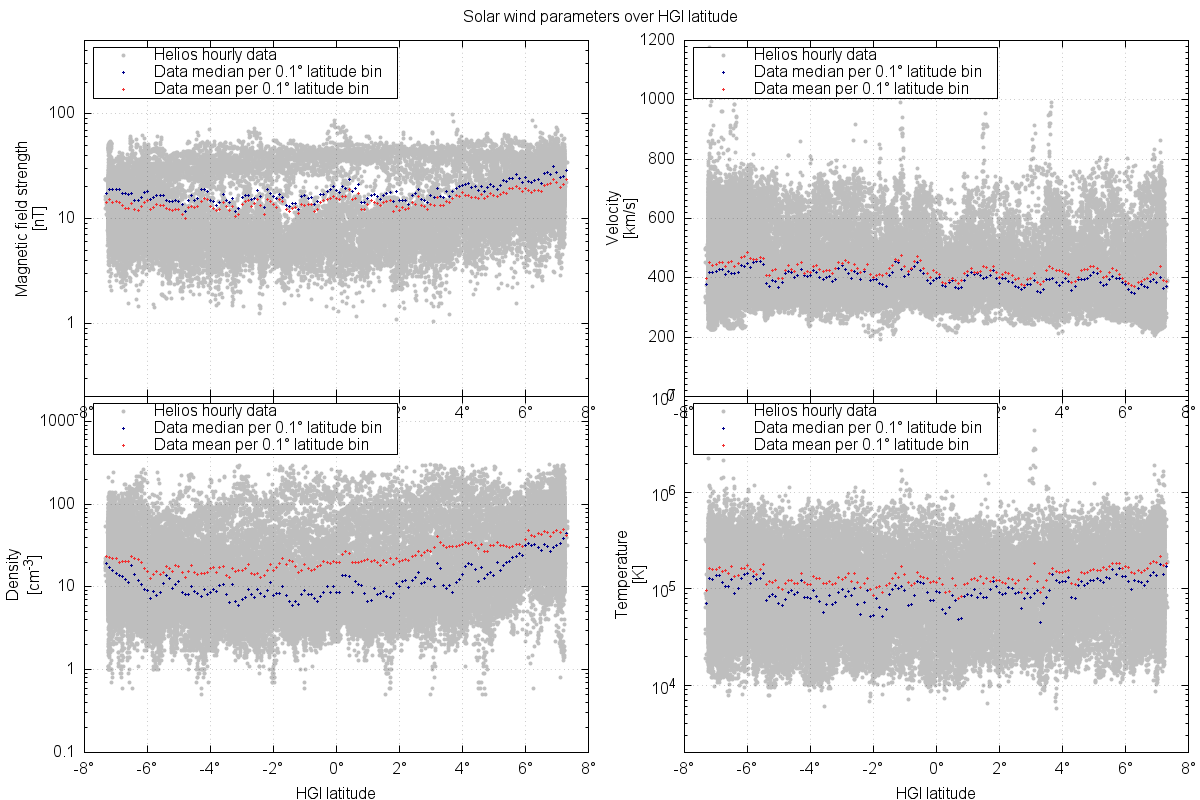
\includegraphics[width=0.5\textwidth]{images/gnuplots/latitude_frequency_4_thesis_plot.png}
	\caption{The four solar wind parameter's HGI latitude dependency. Their mean values per 0.1° bin are plotted as well. make figure same dimensions as projected figure in analysis part...}
	\label{fig:latitude_frequency_4_thesis_plot}
\end{figure}

with the exponential dependencies to 1~au projected solar wind parameters; there are only small changes with latitude in the range -7.25°--7.25°\\
have a look on distribution widths...\\

dependence from latitude in interval -7.25°--7.25° in Helios data negligible?, see \autoref{fig:latitude_frequency_rcorrected_v3_4_thesis_plot}.
\begin{figure}[htb]
	\centering
	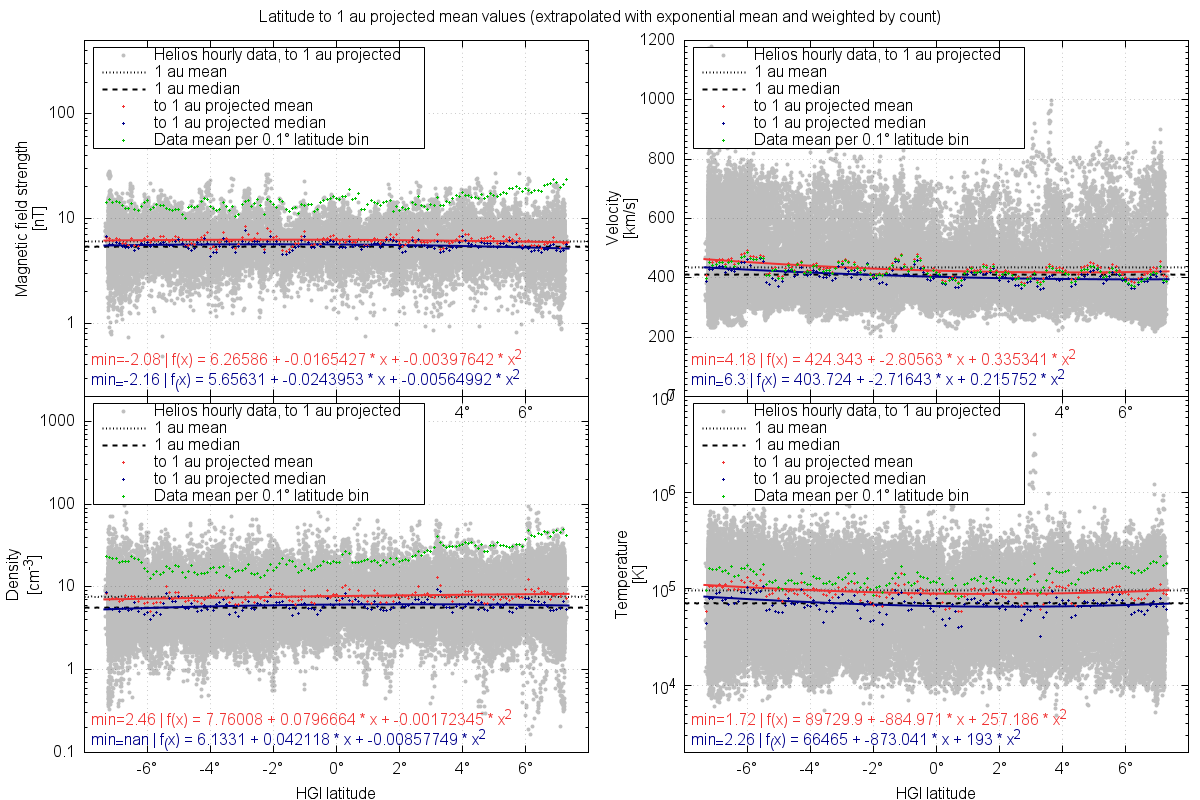
\includegraphics[width=0.5\textwidth]{images/gnuplots/latitude_frequency_rcorrected_v3_4_thesis_plot.png}
	\caption{Plot of the to 1~au projected solar wind parameters over latitude. And their mean values, including weighted fit. add projected median...}
	\label{fig:latitude_frequency_rcorrected_v3_4_thesis_plot}
\end{figure}
estimate error ranges...\\

plot Ulysses data into plot...\\

%latitude variation negligible?
influence from latitude variation in data negligible? (see Ulysses figure in introduction). Helios probes within ecliptic => variation span equal to solar tilt: -7.25° to 7.25°; solar tilt/obliquity to ecliptic: $i_\odot = 7.25\degree$ (Sun fact sheet: \url{http://nssdc.gsfc.nasa.gov/planetary/factsheet/sunfact.html)}\\
big part of Helios data is from latitudes $>\pm5$°, see Figure~XX (data count over latitude) and see Figure~XX (Helios orbit polar plane in data section...)\\


\section{Radial evolution of solar wind structures}
%see CGAUSS report2015_2

Helios event lists HSSs, SLOWs, CIRs, CMEs...; event lists for all Helios data\\
see Liu2004 for Helios ICME list and radial dependencies of B, n, T and v...\\

200~km/s slow solar wind at 10~$R_\odot$ is in agreement with blob measurements from Wang2000\\

very slow sw (VSSW) gets accelerated; see Sanchez-Diaz2016:\\
%"The reported in situ measurements suggest that the properties of VSSW are a continuation of the slow wind toward lower speeds: higher densities, higher proton fluxes, and lower temperatures, thereby extending well-known scaling laws [Lopez and Freeman, 1986; Hundhausen et al., 1970] down to speeds as low as 200 km/s."\\
%"The VSSW has a number of interesting properties that suggest it may be the interplanetary signature of long HPS crossings."\\

structure extrapolations\\

radial diameter of MCs increase between 0.3~au and 4.3~au proportional to the distance as $r^{0.8}$ \citep{Bothmer1998}\\

MC central axial magnetic field strength radial density dependence $B = 18.1\,r^{-1.64}$ \citet{Leitner2007}\\
MC average diameter $D = 0.23\,r^{1.14}$ \citet{Leitner2007}

sw structure marked plot\\


\section{Solar distance dependency---theory}
B-field radial profile: $B \propto r^{-1.5?}$\\
	Magnetic field magnitude model (Kivelson 1995):\\
	Br(r) = B0 / r²\\
	Bphi(r) = -B0 omega / (Vr * r) (shear effect from solar rotation omega)\\
	Btheta(r) = 0\\
	B(r) = (Br² + Bphi² + Btheta²)**1/2\\
	see also \url{radial_fit_B_test_plot.png}\\
	Parker references\\
velocity radial profile: $V \propto r^{0?}$\\
	model based on LeBlanc1998 electron density with flux conservation: Zic2015(Temmer)\\
density radial profile: $N \propto r^{-2}$\\
	simple view: for a spherical constant velocity mass outflow a one over distance squared law is expected, because of the mass flux conservation per solid angle for different distances. measurements up to the outer heliosphere confirm the $1/r^2$ dependency (1--38~au by Voyager~2, \citep{Belcher1993} newer paper?)\\

	in an ideal neutral plasma the electron and proton number density have the same values (neutral plasma) (reference?)\\
	ca. 10~\% more electrons than protons (due to alphas) cite?\\	%http://omniweb.gsfc.nasa.gov/ftpbrowser/bow_derivation.html\\
temperature radial profile: $T \propto r^{-1?}$\\
	at larger distances heating outbalances the adiabatic temperature part (adiabatic cooling vs. pickup proton and stream--interaction heating; 1--68~au by Voyager~2; \citet{Richardson2003}\\
solar wind ram pressure $p_\text{ram} = \rho V^2$\\

\section{flux conservation}
conserved quantities:\\
- momentum conservation... VBbookp112\\
- flux conservation...\\

%%%%%%%%%%%--  flux  --%%%%%%%%%%%%%%%
%As Schwenn1983 stated ``From Helios in situ measurements we know that at least beyond 0.29~au there is almost no nonradial flow, on the average. In fact, the particle flux was found to be that quantity which varies the least with increasing R.''\\

%Schwenn1990:
%increase in sw velocity with distance; speed increase mainly in slow solar wind
%density deviates from a purely r^-2 fall-off (10% faster); n(r)=6.1*r^-2.1 cm^-3; different behavior in slow and fast wind
%proton flux density constant between 0.3-1.0~au -> no meridional flow into/out of the ecliptic; different for slow and fast sw

With consideration of continuity the mass flux per solid angle has to be constant: $\dot{m} = \text{const}$\\
conserved quantities:\\
- mass flux: $\dot{m} = \rho v A$ (with mass density $\rho$, velocity $v$ and [cross-sectional area $A$] or solid angle?...)\\
- particle fluxes (proton flux, electron flux, etc.)\\
	- proton flux: $j_\text{p} = n_\text{p} v_\text{p} A$ (with proton density $n_\text{p}$ and proton velocity $v_\text{p}$)\\

(with proton mass density $\rho = n_\text{p} m_\text{p}$ (with proton number density $n_\text{p}$ and proton mass $m_\text{p}$).)\\

the individual radial dependencies for a spherical radial outflow are:\\
$A(r) \propto r^2$ --> $A/r^2 = \text{const}$\\
and assuming an exponential dependency,\\
$n_{\text{p}}(r) = n_0 r^{c_n}$,\\
$v(r) = v_0 r^{c_v}$\\
\begin{align}
	j_\text{p} &= \text{const}\\
	n_\text{p} v_\text{p} A &= \text{const}\\
	n_0 r^{c_n} v_0 r^{c_v} r^2 &= \text{const}\\
	r^{c_n} r^{c_v} r^2 &= \text{const}\\
	\Rightarrow c_n + c_v + 2 &= 0\\
	c_n + c_v &= -2
\end{align}
an increasing velocity should result in a steeper density...\\

validity of mass flux continuity: within the heliosphere mass to energy conversion and vice versa is negligible, but there can be flux from and to higher latitudes as the Helios data is localized to a small latitude range in the ecliptic plane.\\
estimate the error from that... (if error is too big => drop continuity condition)\\
larger errors should be located near CMEs and CIRs (nonradial flows from interactions)\\
there is a proton flux difference between slow and fast solar wind streams (see book Schwenn1990 p.~146)

estimate the possible size of error:\\
mean:\\
$c_n = -2.010$\\
$c_v = 0.049$\\
$c_n + c_v = -1.961$\\
difference to -2 is 0.039\\
% [median:\\
% $c_n = -2.093$\\
% $c_v = 0.058$\\
% $c_n + c_v = -2.035$\\
% difference to -2 is -0.035\\
% ]constant mass flux only for mean...\\

\section{sw parameters and precision}
definition of 'the four solar wind parameters':\\	%by OMNI histograms
	magnetic field strength, aka magnetic field, $B$, usually measured in nT, in the order of 0--35~nT at 1~au\\
	proton bulk velocity, aka velocity, $v$, usually measured in km/s, in the order of 200--900~km/s at 1~au\\
	proton number density, aka density, $n$, usually measured in cm$^{-3}$, in the order of 1--60 at 1~au\\
	proton temperature, aka temperature, $T$, usually measured in K, in the order of 10\,000--1\,000\,000~K at 1~au\\
sentence about ordering of the parameters...\\

%data binning
hourly OMNI data\\
measurement precision:\\
$B$: 0.01~nT\\
$v$: 1~km/s\\
$n$: 0.1~cm$^{-3}$\\
$T$: 1~K ? (smallest found: 7~K)\\

error discussion:\\
OMNI hourly data mean:\\
$B$: bin size 0.5~nT, median 5.6, mean 6.30056(18)\\
$v$: bin size 10~km/s, median 414, mean 437.6700(18)\\
$n$: bin size 1~cm$^{-3}$, median 5.3, mean 6.831410(18)\\
$T$: bin size 10\,000~K, median 80\,751, mean 112\,219.0(19) (with 1000~K as precision)\\

empirical data; Helios; hourly\\
why hourly and not higher resolution data?\\
measurement precision:\\
$B$: 0.01~nT\\
$v$: 0.1~km/s\\
$n$: 0.1~cm$^{-3}$\\
$T$: 100--1000~K (3 digits)\\
$r$: 0.01~au\\

error discussion:\\
Helios hourly data mean:\\
$B$: min 337, precision: 0.000545; 18.3x better\\
$v$: min 497, precision: 0.00449; 22.2x\\
$n$: min 497, precision:  0.00449; 22.2x\\
$T$: min 497, precision: 4.49--44.49 22.2x\\
=> so we use 1/10 the measurement precicion for the mean.\\

median precision same as data precision\\

%data binning
Helios histogram bin size for mean of frequency distribution (at specific solar distance)\\
$B$: bin size 0.5~nT, min 337, mean precision: 0.000545\\
$v$: bin size 1~cm$^{-3}$, min 497, mean precision: 0.00449\\
$n$: bin size 10~km/s, min 497, mean precision:  0.00449\\
$T$: bin size 10\,000~K, min 497, mean precision: 4.49--44.49\\

\section{other}
McGregor2011 analyzed the empirical magnetic topology–velocity relationship, using Helios perihelion data with the Wang-Sheeley-Arge (WSA) coronal model, and found indications, that the fast and slow solar wind are generated from distinct sources. (not only superradial expansion)\\


Larger individual graphs can be found in the appendix...

state this at the first occurence... (from GUM guide)\\
mS = 100,021 47(35) g, where the number in parentheses is the numerical value of (the combined standard uncertainty) uc referred to the corresponding last digits of the quoted result.\\

%\captionsetup{width=0.75\textwidth}
%align caption width with table width  OR  widen table to textwidth?

For more on lognormal distributions see appendix \autoref{sec:lognormal_distribution}\\

%gnuplot:
%sum of the squared differences or 'residuals' (SSR) between the input data points and the function values, evaluated at the same places. This quantity is often called 'chisquare' 
%'stdfit', the standard deviation of the fit, which is the rms of the residuals, and the variance of the residuals, also called 'reduced chisquare' when the data points are weighted.
%The 'sum of squares of residuals', also called 'chisquare', is the WSSR between the data and your fitted function; fit has minimized that.
%The WSSR can be used to calculate the reduced chisquare (WSSR/ndf) or stdfit, the standard deviation of the fit, sqrt(WSSR/ndf). Both of these are reported for the final WSSR.

we get the ultimate monster equation:\\
\begin{align}
	W_\text{II}(x,\tilde{a}_1, \tilde{b}_1, \bar{a}_1, \bar{b}_1, \tilde{a}_2, \tilde{b}_2, \bar{a}_2, \bar{b}_2) =\\
	\frac{c}{2 \sqrt{\pi \ln\left(\frac{\bar{a}_1 \, r^{\bar{b}_1}}{\tilde{a}_1 \, r^{\tilde{b}_1}}\right)} \, x} \, \exp\left(- \frac{\ln^2\left(\frac{x}{\tilde{a}_1 \, r^{\tilde{b}_1}}\right)}{4 \ln\left(\frac{\bar{a}_1 \, r^{\bar{b}_1}}{\tilde{a}_1 \, r^{\tilde{b}_1}}\right)}\right) + \frac{(1 - c)}{2 \sqrt{\pi \ln\left(\frac{\bar{a}_2 \, r^{\bar{b}_2}}{\tilde{a}_2 \, r^{\tilde{b}_2}}\right)} \, x} \, \exp\left(- \frac{\ln^2\left(\frac{x}{\tilde{a}_2 \, r^{\tilde{b}_2}}\right)}{4 \ln\left(\frac{\bar{a}_2 \, r^{\bar{b}_2}}{\tilde{a}_2 \, r^{\tilde{b}_2}}\right)}\right)
\end{align}

\begin{figure}[htb]
	\centering
	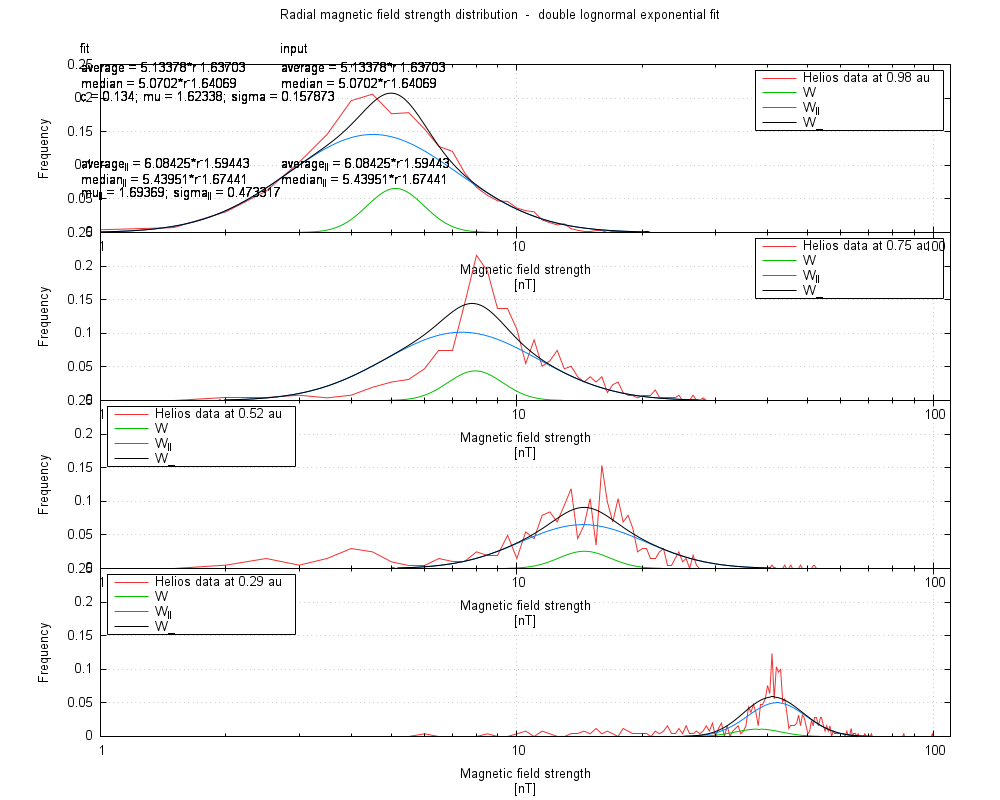
\includegraphics[width=0.4\textwidth]{images/gnuplots/double_fit_B_freq_r_plot_thesis.png}
	\caption{Plot of the magnetic field strength's frequency distribution at different solar distances (0.29, 0.52, 0.75 and 0.98~au). The Helios data, the composed fit model and both its components are plotted. 0.23~au steps, lw 2, stepfunction}
	\label{fig:double_fit_B_freq_r_plot_thesis}
\end{figure}

=> what kind of distribution has the B-field near the Sun?\\

The extrapolation distance is only about one third of the model range, but as the parameters follow exponential change, one has to look at the logarithmic distance which is indeed one and a half times the model range.\\

argument with gravitational deceleration; near-Sun extrapolation should be biased, because in the near-Sun region gravitation becomes significant (see \autoref{fig:v_vs_r_b})\\
\begin{figure}[htb]
	\centering
	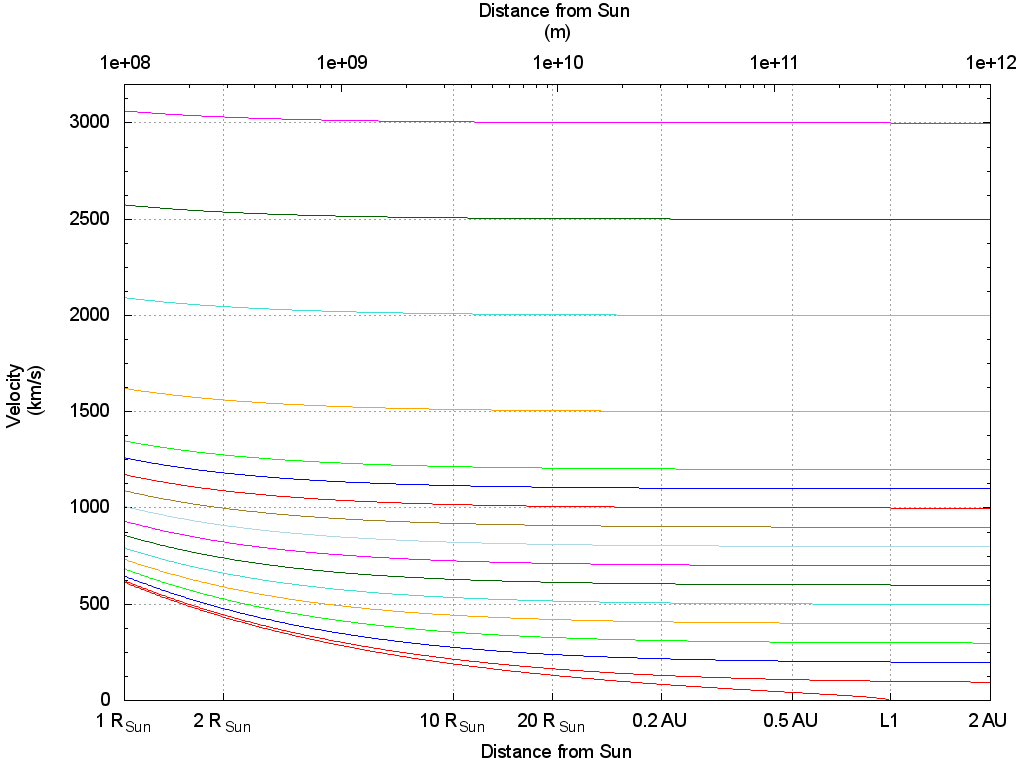
\includegraphics[width=0.3\textwidth]{images/gnuplots/v_vs_r_b.png}
	\caption{velocity over solar distance; gravitational deceleration. place instead figure of grav. force over solar distance...}
	\label{fig:v_vs_r_b}
\end{figure}


comparison...\\
...with Vourlidas estimates at 10~$R_\odot$\\
...with Wang2000 slow blobs\\

